\label{I2CAdapter}

Aufgrund der hohen PIN-Belegung des \ac{LCD}-Displays und den damit fehlenden digitalen Steckmöglichkeiten am Arduino, haben wir uns dazu entschieden, den in Abbildung \ref{fig:I2CAdapter} zu sehenden I$^2$C-Adapter, zu verwenden. \\
Mit diesem Adapter ist es nun möglich, sechs digitale PINs, welche wir vorher hätten verwenden müssen, auf zwei analoge PINs zu reduzieren. Somit reichen die digitalen PINs am Arduino für drei Taster, einen CO2-Sensor und eine Mikro-SD-Karten Adapter auf jeden Fall aus.

\begin{figure}[!hbt]
	\centering
	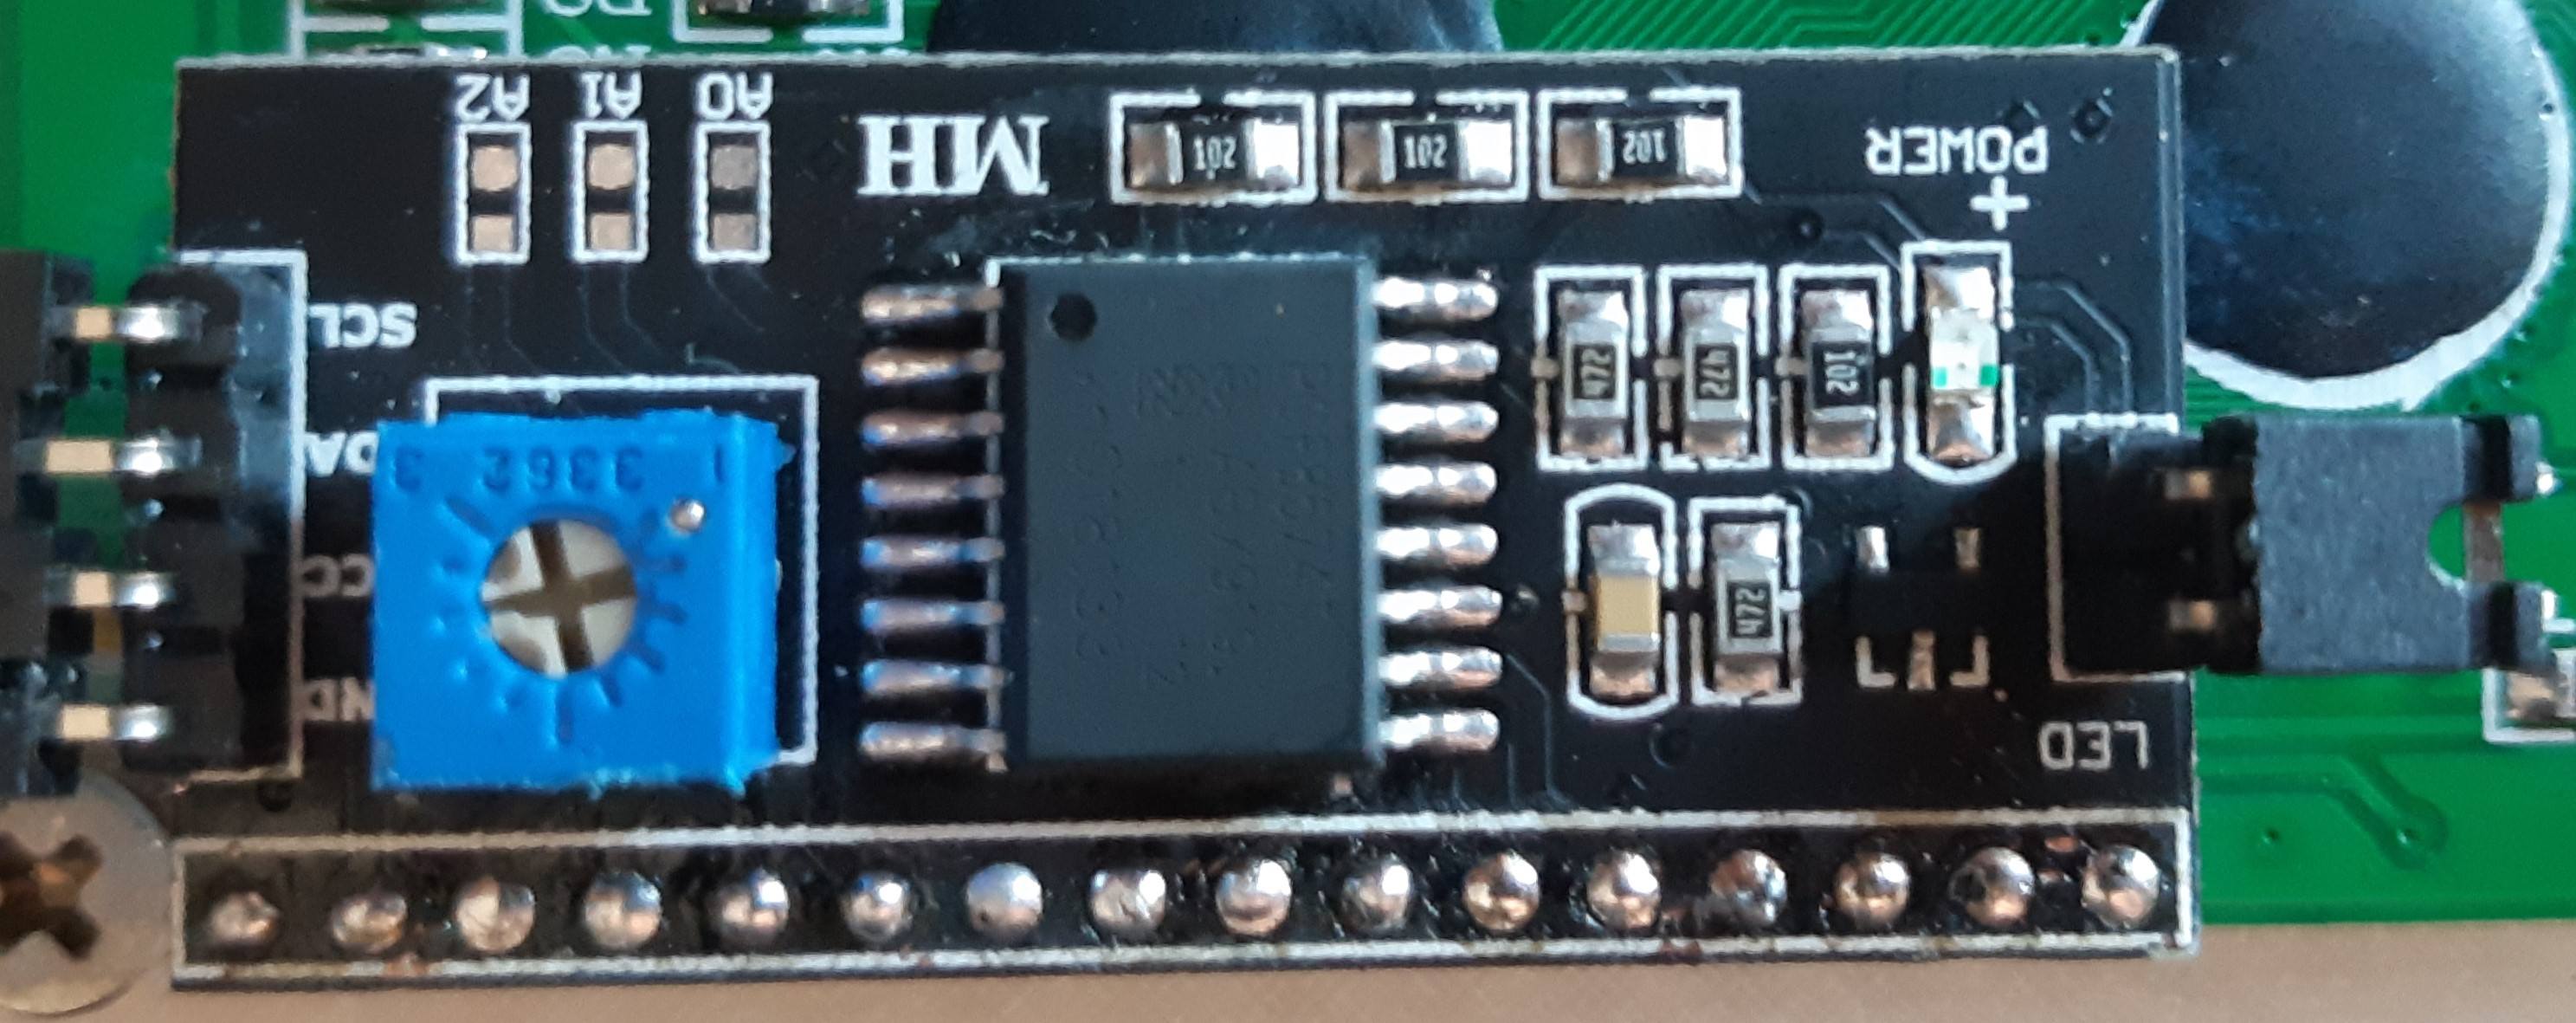
\includegraphics[width=0.5\linewidth]{Images/I2CAdapter}
	\footnotesize \\Quelle: eigene Aufnahme
	\caption{Verwendeter I$^2$C-Adapter}
	\label{fig:I2CAdapter}
\end{figure}

Die Implementierung des I$^2$C-Adapters erfolgt über die Bibliothek <LiquidCrystal\_I2C.h>. In dieser können die gleichen Befehle aufgerufen werden, welche schon in der Bibliothek <LiquidCrystal.h> genutzt werden konnten. Die restlichen Befehle funktionieren mit beiden Bibliotheken. Somit muss bei einer späteren Umrüstung nur wenig im Quellcode geändert werden. Die einzige Änderung muss bei der Adressvergabe und Größenangabe des \ac{LCD}-Displays vorgenommen werden. \\
So konnten die Adressen am Arduino vorher durch das aneinanderreihen der digitalen PINs im Quellcode definiert werden. Zudem gab es im Setup eine weitere Zeile, in welcher die Anzahl der Zeichen und Reihen des Displays angegeben werden musste. \\
In Abbildung \ref{fig:I2CAdressen} ist der Codeausschnitt zu sehen, welcher zum einen die Adressen definiert, zum anderen aber auch angibt, wie viele Zeichen und Reihen verwendet werden sollen. \\
Durch drehen des Rades am grau-blauen Aufsatz, welcher in Abbildung \ref{fig:I2CAdapter} links im Bild zu sehen ist, wird der Kontrast eingestellt. Ein Vorwiderstand muss somit nicht händisch zwischen Arduino und \ac{LCD}-Display geschaltet werden.

\begin{figure}[!hbt]
	\centering
	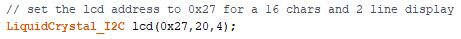
\includegraphics[width=0.6\linewidth]{Images/I2CAdressen}
	\footnotesize \\Quelle: eigene Aufnahme
	\caption{Codeausschnitt zur Definition von Adresse und Anzahl der zu verwendenden Zeichen und Reihen}
	\label{fig:I2CAdressen}
\end{figure}
